\documentclass[../../main.tex]{subfiles}

\begin{document}

Assuming the tree $T$ created above is accurate, we now seek to infer genotypes from this phylogeny so as to overcome errors and noise associated with low coverage SCS data.
We first determine weights for attaching point mutations and different types of LOH events to different edges of the tree, and then use these weights to determine genotype probabilities for each cell.
The approximate phylogeny was found by combing information from across the genome, however to infer cell genotypes we shall return to considering individual loci.

\subsubsection{SNV weights}
In the simplest case, we ignore any potential loss of heterozygosity.
For each edge of the tree $e$, we seek to answer the following question: assuming there is a pont mutation at this locus, what is the probability it occurred at $e$?

To begin with, we compute the likelihood of all descendents of an edge in the tree having the same genotype.
We say that $\pi_0(e), \pi_1(e)$ and $\pi_2(e)$ are respectively the likelihoods that all descendents of $e$ are homozygous reference, heterozygous and homozygous alternate.

These values are taken to be
\begin{equation}
\pi_g(e) = \prod_{\{j:c_j\succ e\}} P(g_j = g)
\end{equation}
where $c_j\succ e$ indicates that the $j^{th}$ cell is below $e$ in $T$.
$P(g_j = g)$ here are the probabilities calculated in Equation~\eqref{eq:sitebayes}.
We also compute one more value, $\pi_\mu(e)$, defined as the likelihood that all descendents of $e$ have a genotype of either 1 or 2, that is to say they are mutant.
These four values can be computed recursively in $O(m)$ time by multiplying the corresponding values from the two branches directy beneath each branch.

If an SNV occurred at edge $e$ in $T$, we would expect that all descendents of $e$ would have genotypes of 1 or 2, while all other cells would have genotype 0 (assuming infinite sites).
Letting $\rho$ be the edge ancestral to all sampled cells, it is easy to verify that the likelihood of this simplifies to:
\begin{equation*}
    \prod_{c_x\succ e}P(g_x =1,2)\prod_{c_x\nsucc e} P(g_y = 0) = \pi_\mu(e)\frac{\pi_0(\rho)}{\pi_0(e)}
\end{equation*}
The prior probability of a mutation occuring on any branch of the tree can be found by using the edge lengths: mutations occur on longer edges more frequently.
We must undo the Jukes-Cantor correction that was useful for neighbor joining to find a value proportional to the expected number of SNVs along an edge.
We find $\overline{p}_e = \frac{3}{4}\left(1-e^{-\frac{4}{3}d_e}\right)$ to be such a value and therefore define the prior probability of attaching a SNV to edge $e$ to be:
\begin{equation*}
    P(S_e) = \frac{\overline{p}_e}{\sum_{e'}\overline{p}_{e'}}
\end{equation*}
Since $\pi_0(\rho)$ and $\sum_{e}\overline{p}_{e}$ are constant for a locus, we define a weight for attaching a SNV with no LOH to edge $e$ as:
\begin{equation*}
    W(S_e) = \frac{\pi_\mu(e)}{\pi_0(e)} \overline{p}_e
\end{equation*}
which is proportional to the posterior probability of attachment at $e$ (assuming a SNV occurred at this locus) up to a normalization constant.
When we recurse up the tree computing $\pi_g$ values, we can also compute and store these weights $W(S_e)$.
If we recursively sum the weights from the two childen of each node, at the root this sum value will equal the total sum of weights and we can thereafter derive the probabilities:
\begin{equation} \label{eq:SNVattachP}
    P(S_e\,\mid\,SNV) = \frac{W(S_e)}{\sum_{e'}W(S_e)}
\end{equation}


\subsubsection*{Weights For Loss of Heterozygosity}

\begin{figure}[h]
	\centering

	\begin{subfigure}{0.2\textwidth}
		\centering
		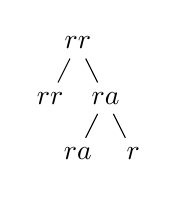
\begin{tikzpicture}[sibling distance=2em, level distance=2em]
  \node {$rr$}
    child { node {$rr$} }
    child { node {$ra$}
      child { node {$ra$} }
      child { node {$r$}}
          };
		\end{tikzpicture}
		\caption{Case 1}
	\end{subfigure}
	\begin{subfigure}{0.2\textwidth}
		\centering
		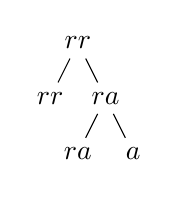
\begin{tikzpicture}[sibling distance=2em, level distance=2em]
  \node {$rr$}
    child { node {$rr$} }
    child { node {$ra$}
      child { node {$ra$} }
      child { node {$a$}}
          };
		\end{tikzpicture}
		\caption{Case 2}
	\end{subfigure}
	\begin{subfigure}{0.2\textwidth}
		\centering
		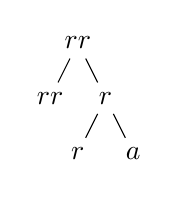
\begin{tikzpicture}[sibling distance=2em, level distance=2em]
  \node {$rr$}
    child { node {$rr$} }
    child { node {$r$}
      child { node {$r$} }
      child { node {$a$}}
          };
		\end{tikzpicture}
		\caption{Case 3}
	\end{subfigure}
	\begin{subfigure}{0.2\textwidth}
		\centering
		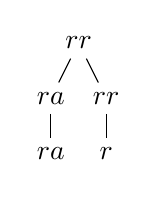
\begin{tikzpicture}[sibling distance=2em, level distance=2em]
  \node {$rr$}
    child { node {$ra$} 
    	child { node {$ra$} }
    	  }
    child { node {$rr$} 
    	child { node {$r$} }
    	};
		\end{tikzpicture}
        \caption{Case 4}
    \end{subfigure}
    \caption{Different ways loss of heterozygosity can occur in a tree.}
    \label{fig:treecases2}
\end{figure}

The more complicated cases invlove both a SNV and a ploidy change occuring at the same locus.
The four possible ways this can occur is shown in Figure~\ref{fig:treecases2}.

For case 1, a point mutation occurred at edge $e_1$ before a ploidy change dropped the alternate allele at $e_2$.
We expect that all cells $e\succ e_2$ will have genotype 0; cells for which $e\succ e_1$ but $e\nsucc e_2$ will have genotype 1 and all other cells will have genotype 0.
Similar to the simplest case, the likelihood of a SNV at $e_1$ followed by a dropped alternate allele at $e_2$ is given by:
\begin{equation*}
    \prod\limits_{c_x\succ e_2}P(g_x = 0)\times\prod\limits_{c_y\succ e_1,\nsucc e_2} P(g_y = 1)\times\prod\limits_{c_z\nsucc e_1, \nsucc e_2} P(g_z=0)
    = \pi_0(e_2)\cdot\frac{\pi_1(e_1)}{\pi_1(e_2)}\cdot\frac{\pi_0(\rho)}{\pi_0(e_1)}
\end{equation*}

The prior probability of attaching the SNV at $e_1$ is the same as in the simple case: normalized $\overline{p}_{e_1}$.
The prior probability of attaching a loss of heterozygosity at $e_2$, however, is subtly different.
We assume that a loss of heterozygosity affecting just a single cell is far less probable than an allelic dropout event during the amplification process.
Therefore we define
\begin{equation*}
    P(L_{e}) = \frac{\overline{p}_e}{\sum_{e'\in E-E_L}\overline{p}_{e'}}
\end{equation*}
where $E_L$ is the set of all edges directly above a leaf node.
This is the same as setting the prior probability of a loss of heterozygosity affecting individual cells to 0.
The weight of attaching the SNV to $e_1$ and the LOH to $e_2\succeq e_1$ for case 1 is:
\begin{equation}
    W^{(1)}(S_{e_1},\,L_{e_2}) = \frac{\pi_0(e_2)\pi_1(e_1)}{\pi_1(e_2)\pi_0(e_1)}\overline{p}_{e_1}\overline{p}_{e_2}
\end{equation}
Assuming both a SNV and LOH have occurred at the locus, and the case is case 1, this weight can be converted into a joint attachment probability by normalizing over the pairs of edges for which $\{e_1,e_2\}\subset E-E_L$ and $e_1\preceq e_2$.

The weights for cases 2 and 3 can be found using similar logic to be:
\begin{equation}
    W^{(2)}(S_{e_1},\,L_{e_2}) = \frac{\pi_2(e_2)\pi_1(e_1)}{\pi_1(e_2)\pi_0(e_1)}\overline{p}_{e_1}\overline{p}_{e_2}
\end{equation}
\begin{equation}
    W^{(3)}(S_{e_1},\,L_{e_2}) = \frac{\pi_2(e_1)}{\pi_0(e_1)}\overline{p}_{e_1}\overline{p}_{e_2}
\end{equation}
although $W^{(3)}$ has the slightly different domain for normalization: $e_2\in E-L,\,e_1\in E$ and of course $e_1\succeq e_2$.

\subsubsection*{Marginal Probabilities of Ploidy Change}

For cases 1 and 2, it will be useful to answer the following question at each edge: assuming there is a case $i$ event at this locus and a SNV has already been observed ancestral to this edge, what is the probability that a LOH event will happen at this edge?
Let us assume that an SNV occurs at this locus and that a case 1 loss of heterozygosity also definitely occurs.
We first see that for any $e'\preceq e$: 
\begin{align*}
    P(L_e\,\mid\,S_{\preceq e}) &= \frac{P(L_e\cap S_{\preceq e})}{P(S_{\preceq e})}\\
    &= \frac{P(L_e\cap(S_\rho \cup S_{e_i} \cup \dots)}{P(S_\rho \cup S_{e_i} \cup \dots)}\\
    &= \frac{P((L_e\cap S_\rho) \cup (L_e\cap S_{e_i}) \cup \dots)}{P(S_\rho \cup S_{e_i} \cup \dots)}
\end{align*}
Due to infinite sites, mutations on different branches at a locus are mutually exclusive, hence
\begin{equation*}
    P(L_e\,\mid\,S_{\preceq e}) = \frac{\sum_{e'\preceq e}P(L_e\cap S_{e'})}{\sum_{e'\preceq e}P(S_{e'})}
\end{equation*}
The numerator is a sum over the joint attachment probability distribution for case 1 given by $W^{(1)} (S_{e'},\,L_e)$ and the denominator is a sum over the distribution found in Equation~\ref{eq:SNVattachP}.

To compute the various values of $W^{(1)}(S,\, L)$ we can traverse the tree and at each edge $e$ (excluding edges above a leaf)  sum the values of $W^{(1)}(S_{e'\preceq e},\,L_e)$, as well as $P(S_e'\preceq e)$.
This traversal takes $O(m\log m)$ time in the best case, and $O(m^2)$ in the worst case.
Summing all these partial sums  of $W^{(1)}$ will give us the normalization constant which can be divided out afterwards.

This has all been shown assuming case 1 to be true for the locus, but the values for case 2 are exactly similar and can be computed in the same traversal.
Case 3, however, is somewhat different, as we need to find the probability of an LOH given that no ancestral edge has a SNV:
\begin{align*}
    P(L_e\,\mid\,\neg S_{\prec e}) &= \frac{P(L_e\cap S_{\succeq e})}{P(\neg S_{\prec e})}\\
   &= \frac{1}{\sum W^{(3)}}\cdot\frac{\sum_{e'\succeq e}W^{(3)}(S_{e'},\,L_e)}{\prod_{e'\prec e}\left[1-P(S_{e'})\right]}
\end{align*}
Calculating this value at each node requires values from all ancestors and descendants, and therefore can only be calculated in $O(m^2)$.

The marginal probabilities here have so far assumed not only that there is a loss of heterozygosity at the locus, but also that their particular case is true.
We established when determening prior probabilities for $\sigma$ that 

%OLD:
\newpage
Referring to Figure~\ref{fig:treecases2} above these weights are calculated for cases 1, 2 and 3 in the following way:
\begin{equation*}
W^{(1)}(S_{e_1},L_{e_2}) = \frac{\pi_0(e_2)\pi_1(e_1)}{\pi_1(e_2)\pi_0(e_1)}d_{e_1}P(L_{e_2})
\end{equation*}
\begin{equation*}
W^{(2)}(S_{e_1},L_{e_2}) = \frac{\pi_2(e_2)\pi_1(e_1)}{\pi_1(e_2)\pi_0(e_1)}d_{e_1}P(L_{e_2})
\end{equation*}
and
\begin{equation*}
W^{(3)}(S_e) = \frac{\pi_2(e)}{\pi_0(e)}d_e
\end{equation*} 
If a haploid event should occur at the locus under examination, the prior probability that it should occur on edge $e$ is given to be: %TODO may need to lengthen root edge to account for homozygous alternate germline mutations
\begin{equation*}
P(L_e) = \frac{d_e}{\sum_{e'\in E-E_l} d_{e'}}
\end{equation*}
where $E_l$ is the set of all edges directly above leaf nodes. It is assumed that allelic dropout due to amplification is much more frequent than ploidy changes that affect only a single cell, and thus the prior probability of the latter is set to 0. For cases 1 and 2 we define
\begin{equation*}
W'^{(1)}(L_e) = \frac{\sum_{e' \preceq e} W^{(1)}(S_{e'},L_e)}{\sum_{e' \preceq e}W(S_e')} 
\end{equation*}
where the values in the denominator come from Equation~\eqref{eq:Wmu}. Similarly
\begin{equation*}
W'^{(2)}(L_e) = \frac{\sum_{e' \preceq e} W^{(2)}(S_{e'},L_e)}{\sum_{e' \preceq e}W(S_e')} 
\end{equation*}
%TODO this assumes LOH and SNV positions are independent. Is this biased for those highr or lower or neither?
Finally, assuming an SNV has already occured at the given locus, the probability of a case 1 haploid event happening at any edge $e$ is given by (see appendix ??):
\begin{equation*}
P(L_e^{(1)}) = P(L_e^{(1)}\mid S_{\preceq e}) = \frac{P(LOH)}{3} \frac{W'^{(1)}(L_e)}{\sum_{e'\in E-E_l}W'^{(1)}(L_{e'})}
\end{equation*}
and under the same assumption, the conditional probability for case 2:
\begin{equation*}
P(L_e^{(2)}) = P(L_e^{(2)}\mid S_{\preceq e}) = \frac{P(LOH)}{3} \frac{W'^{(2)}(L_e)}{\sum_{e'\in E-E_l}W'^{(2)}(L_{e'})}
\end{equation*}
The probability for case 3 is given by
\begin{equation*}
P(L_e^{(3)}) = P(L_e^{(3)}\mid S_{\preceq e}) = \frac{P(LOH)}{3} \frac{W^{(3)}(L_e)}{\sum_{e'\in E-E_l}W^{(3)}(L_{e'})}
\end{equation*}
The prior probability $P(LOH)$ of a loss of heterozygosity occuring at the site given that a SNV has occured is given to be
\begin{equation*}
P(LOH) = P(LOH_i \mid SNV_i) = \frac{3}{2}\cdot\frac{1-\prod_j\left[P(g_{ij}=0)+P(g_{ij}=1)\right]}{1-P(\sigma_i = 0)}
\end{equation*}

\subsubsection*{Genotyping Cells}
%TODO got to keep a running probability of case 3, separate from genotype probs. prob of 2 from 0 = p(S_e)*(sum(P(case 3 ancestral))+case2 at e)
With all of these values computed for each of the edges in the tree, we can use a dynamic programming algorithm to genotype the cells. We complete a depth first traversal of the tree keeping track of genotype probabilities at every node. We also keep track of the probability $P(L_{\preceq e}^{(3)})$ that a silent case 3 haploid event has occured ancestral to each node. The initial conditions for the root node are the genotype probabilities $P(g=0)=1$ and $P(g=1)=P(g=2)$ and $P(L_{\preceq \rho}^{(3)}) = 0$. Let $n_1$ be the direct ancestor of $n_2$ such that $n_1$ and $n_2$ are joined by $e$ and have genotypes $g_1$ and $g_2$ respectively. Therefore we define the relations:
\begin{equation*}
P(L^{(3)}_{\preceq n_2}) = P(L^{(3)}_{\preceq n_1}) +P(L^{(3)}_e)
\end{equation*}
\begin{align*}
P(g_2 = 0) = &P(g_1=0)\left[(1-P(S_e))+P(S_e)P(L^{(1)}_e)\right]\\
+ &P(g_1 = 1)\left[P(L^{(1)}_e)\right]
\end{align*}
%TODO is it necessary to include that no type 3, is that assumed?
\begin{align*}
P(g_2 = 1) = &P(g_1=0)\left[P(S_e)(1-P(L^{(1)}_e)-P(L^{(2)}_e))\right]\\
+ &P(g_1 = 1)\left[1-P(L^{(1)}_e)-P(L^{(2)}_e)\right]
\end{align*}
%TODO do we need 1-P(S_e) here?
\begin{align*}
P(g_2=2) = &P(g_1=0)\left[P(S_e)(P(L^{(3)}_{\preceq n_2}) + P(L^{(2)}_e))\right]\\
+ &P(g_1=1)\left[P(L^{(2)}_e)\right]\\
+ &P(g_1=2)
\end{align*}

When the tree traversal reaches the leaf nodes, these are taken to be the cell genotype probabilities. The cell will be genotyped in accordance with the highest probability.


\end{document}
